\documentclass[fleqn,11pt]{article}

\usepackage[letterpaper,margin=0.75in]{geometry}

\usepackage{amsmath}
\usepackage{booktabs}
\usepackage{graphicx}
\usepackage{listings}

\setlength{\parindent}{1.4em}

\begin{document}

\lstset{
  language=Python,
  basicstyle=\small,          % print whole listing small
  keywordstyle=\bfseries,
  identifierstyle=,           % nothing happens
  commentstyle=,              % white comments
  stringstyle=\ttfamily,      % typewriter type for strings
  showstringspaces=false,     % no special string spaces
  numbers=left,
  numberstyle=\tiny,
  numbersep=5pt,
  frame=tb,
}

\title{Reliable Transport}

\author{Devon Kinghorn}

\date{Feb. 23 2017}

\maketitle

\section{Basic Tests}

Reliable transport is a very simple concept. Make sure that every byte of data is received. 
TCP fulfills its reliability needs by using cumulative acks. 
Whenever a new packet is received that node sends an ACK with the next byte empty in its buffer.
As seen below n2 received byte 6000 from n1 but was missing byte 4000 so it sent an ACK for 4000.
The ACK in this case was also lost so n1's timer fired and n1 retransmitted packet 4.
n2 received packet 4 and then sent an ACK for 7000 because it was the next byte n2 needed.

\begin{lstlisting}
1.0424 n1 (1) received TCP ACK from 2 for 4000 current seq 4000
1.0524 n2 (2) received TCP segment from 1 for 6000
1.0524 n2 (2) sending TCP ACK to 1 for 4000
1.0624 n1 (1) received TCP ACK from 2 for 4000 current seq 4000
2.0416 n1 (1) retransmission timer fired
2.0416 n1 (1) sending TCP segment to 2 for 4000
2.0524 n2 (2) received TCP segment from 1 for 4000
2.0524 application got 3000 bytes
2.0524 n2 (2) sending TCP ACK to 1 for 7000
\end{lstlisting}

When the loss is set to 50\% it takes a long to to transmit, but it is reliable. As seen below,
 a small file can take 15 seconds to transmit because it needs to timeout all the time.

 \begin{lstlisting}
4.0948 application got 1000 bytes
14.0948 n2 (2) sending TCP ACK to 1 for 10000
14.1048 n1 (1) received TCP ACK from 2 for 10000 current seq 8000
14.1048 canceling timer
14.1048 maybe starting timer
14.1048 timer not started

File transfer correct!
 \end{lstlisting}

Below are the results of the experiment to show how lost packets increase the time it takes a file to transfer.
Looking at the results it seems as though every lost packet adds about a second delay to the total transfer time, which makes sense.
Whenever a packet is lost the node must wait a full second before retransmitting.
If two or more packets are lost in a window then it doesn't really make a difference. 
The first packet lost is the only timer that runs, and once it hits a timeout all packets in the window are resent.

Sending the documents with a 50\% loss rate significantly slowed down transmission. 
Multiple packets in a window would be lost and when n1 would retransmit the window of packets some of the packets lost in the previous transmission would be lost again.
It is very inefficient and slow when the loss rate is so high. 

 
\vspace{0.5cm}
\begin{tabular}{cccc}
  \toprule
  File & Window Size & Lossrate & Transmission Time(s)\\
  \midrule
  test.txt & 3000 & 0.0 & 0.0832\\
  test.txt & 3000 & 0.1 & 1.0848\\
  test.txt & 3000 & 0.2 & 1.0848\\
  test.txt & 3000 & 0.5 & 16.104\\
  internet-architecture.pdf & 10000 & 0.0 & 1.084416\\
  internet-architecture.pdf & 10000 & 0.5 & 394.0824\\
  \bottomrule
\end{tabular}

\begin{lstlisting}[title={Network Configuration for Basic Tests}]
# n1 -- n2
#
n1 n2
n2 n1

# link configuration
n1 n2 10Mbps 10ms
n2 n1 10Mbps 10ms
\end{lstlisting}

\vspace{0.5cm}

\section{Fast Retransmit}

Using a timeout to resend packets is very effective but it isn't very efficient when there is significant loss. 
Waiting a full second for a timeout leaves a lot of wasted bandwidth.
To show how this can be improved fast retransmit resends a packet when the sender thinks it was lost.
The sender can assume that a packet was lost when 4 duplicate ACKs are received.
Sending a new packet at this time happens just a bit longer than the round trip time which is a lot faster than the one second timeout used before.
This significantly decreases the send time. 
Below is an example of how retransmit works.
If fast retransmit wasn't turned on then a timer would first fire at time 27.384, almost a second slower than fast retransmit.

\begin{lstlisting}
26.348 n1 (1) received TCP ACK from 2 for 506000 current seq 502000
....
26.3688 n1 (1) received TCP ACK from 2 for 506000 current seq 506000
26.3696 n1 (1) received TCP ACK from 2 for 506000 current seq 506000
26.3704 n1 (1) received TCP ACK from 2 for 506000 current seq 506000
26.3704 retransmitting
26.3704 canceling timer
26.3704 starting timer
26.3704 n1 (1) sending TCP segment to 2 for 506000
....
26.3812 n2 (2) received TCP segment from 1 for 506000
26.3812 application got 7000 bytes
26.3812 n2 (2) sending TCP ACK to 1 for 513000
\end{lstlisting}

For an experiment two simulations were run. Each with 10Mbps connections with a 10ms propigation delay and a loss rate of 20\%.
The difference in load times is significant as seen below.
First is the last lines of output of TCP when fast retransmit is turned on.
Below that is the last few lines of output when fast retransmit is not turned on.

\begin{lstlisting}
0.332816 n2 (2) received TCP segment from 1 for 512000
20.332816 application got 2520 bytes
throughput: 25304.9061183
20.332816 n2 (2) sending TCP ACK to 1 for 514520
20.342816 n1 (1) received TCP ACK from 2 for 514520 current seq 512000
20.342816 canceling timer
20.342816 maybe starting timer
20.342816 timer not started

File transfer correct!
\end{lstlisting}

\begin{lstlisting}
8.086 n2 (2) received TCP segment from 1 for 513000
78.086 application got 1520 bytes
totalDelay: 1.1456
78.086 n2 (2) sending TCP ACK to 1 for 514520
78.096 n1 (1) received TCP ACK from 2 for 514520 current seq 513000
78.096 canceling timer
78.096 maybe starting timer
78.096 timer not started

File transfer correct!
\end{lstlisting}

Fast retransmit decreased the time to transmit by a factor of 3 or 4.
This is because 20\% of packets were lost when sent and for every lost packet without fastretransmit the sender needs to have the timeout fire before retransmitting. 
That is almost a second slower on average than if fast retransmit was on. 
It is true that even with fast retransmit enough packets can be lost for a timer being the only method to restart transmission, but fast retransmit is faster.
I also ran with a window size of 15000 and fast retransmission ran in 7 seconds and not running retransmission still took 50 seconds.
Having a larger window really benefits from fast retransmission because the chances of receiving 4 duplicate ACKs is very high so fewer timeouts are encountered.

\begin{lstlisting}[title={Network Configuration for Fast Retransmit}]
# n1 -- n2
#
n1 n2
n2 n1

# link configuration
n1 n2 10Mbps 10ms
n2 n1 10Mbps 10ms
\end{lstlisting}


\section{Experiments}

Sending packets over TCP does not happen at a deterministic rate. 
Packets are sent upon receiving new packets and sliding the window.
This non-deterministic packet sending rate can cause queueing delay.
An experiment was run to measure the queueing delay and see the effect of window size on queueing delay.
A large file was sent over TCP with a zero loss rate.
The window size varied between 1000 and 20,000 bytes long. 
The network configuration is shown at the end of the section.
Below are two graphs showing the throughput and queueing delay as a function of the window size.

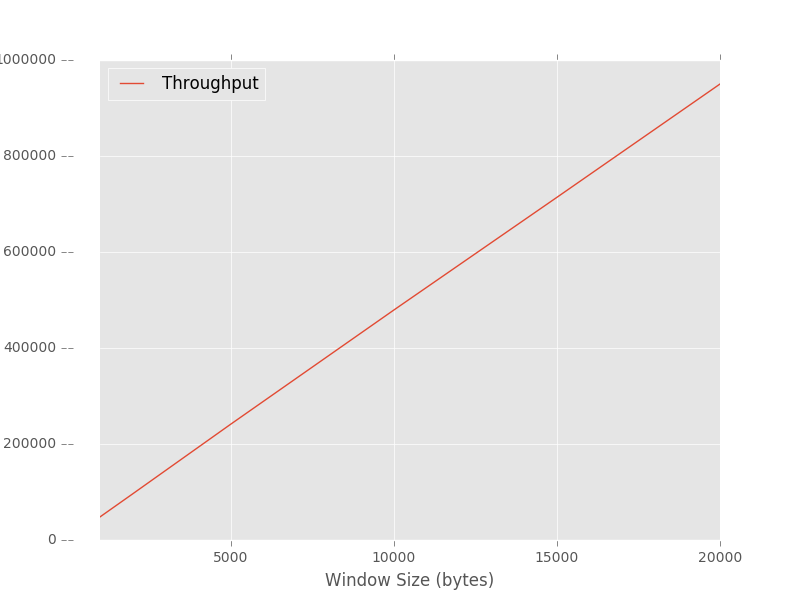
\includegraphics[width=8cm]{throughput.png}
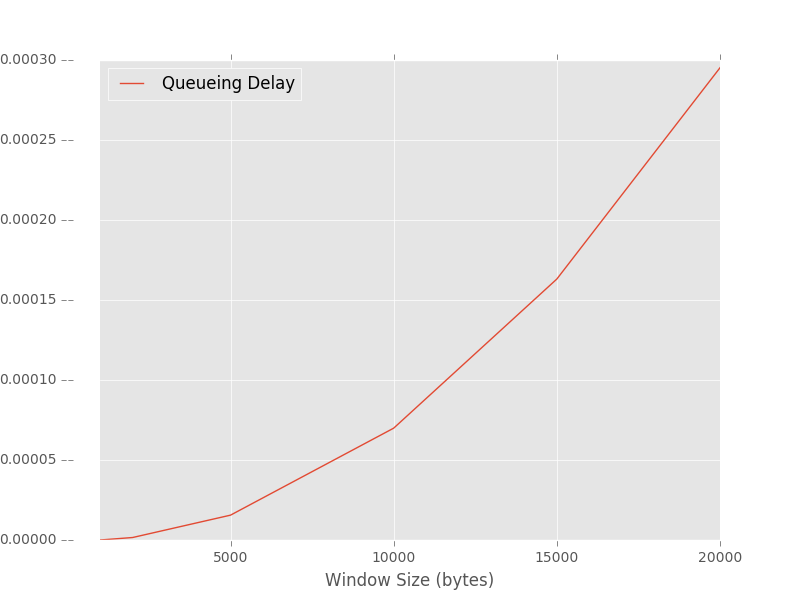
\includegraphics[width=8cm]{delay.png}

The throughput is a linear function of the window size and round trip time. 
\[\text{throughput} = \frac{\text{window  size}}{\text{round trip time}} \]
My experiment shows that in practice this is also true. There is a distinct linear correlation between the window size and the throughput.
My experiment also shows that queueing delay happens as expected.
Packets are sent at a non-deterministic rate.
They are sent in quick volleys before waiting for a volley of ACKs to be returned.
As packets are sent quickly then wait for ACKs to return a queue builds up, even though the service rate is constant.
This queueing pattern matches that of an M/D/1 queue. 

\vspace{0.5cm}

M/D/Q Queue theoretical wait time.

$\bar{w}$ is the average weight time in queue. 

$\rho$ is the average utilization. 

$\mu$ is the service rate.

\[
    \bar{w} = \frac{1}{2\mu}\left(\frac{\rho}{1-\rho}\right)
\]

As the window size increases so does the average utilization $\rho$. 
Queueing theory predicts that as the window size increases the queueing delay should increase exponentially.
This is exactly what happened on the network simulator. 


\begin{lstlisting}[title={Network Configuration for Experiments}]
# n1 -- n2
#
n1 n2
n2 n1

# link configuration
n1 n2 10Mbps 10ms 100packets
n2 n1 10Mbps 10ms 100packets
\end{lstlisting}

\end{document}